
\documentclass[12pt,a4paper,usenames,x11names,compress]{beamer}
\usetheme[numbering=none,block=fill,progressbar=foot]{metropolis}
\useoutertheme{metropolis}
\setbeamercolor{frametitle}{bg=DarkOrange1}
\setbeamercolor{progress bar}{fg=Chocolate1,bg=SkyBlue1}
\setbeamercolor{block title}{fg=white,bg=RoyalBlue4}
\setbeamercolor{block body}{fg=black,bg=SteelBlue4!20}
\setbeamercolor{normal text}{fg=black}
\usepackage{array}
\newcolumntype{P}[1]{>{\centering\arraybackslash}p{#1}}
\usepackage{amsmath}
\usepackage{amssymb}
\usepackage{commath}
%\usepackage{xcolor}
\usepackage{color}
\usepackage[utf8]{inputenc}
\usepackage[english, spanish]{babel}
\usepackage[T1]{fontenc}
\usepackage{lmodern}
\usepackage{ragged2e}
\usepackage{hyperref}
\usepackage{siunitx}
\usepackage{colortbl}
\usepackage{metalogo}
\usepackage{multirow}
\usepackage{tikz}
\usetikzlibrary{shapes.geometric, arrows}
\usetikzlibrary{positioning}
\usetikzlibrary{decorations.pathmorphing,calc,shadows.blur,shadings,mindmap}
\usepackage{smartdiagram}


\tikzset{
  my blur shadow layer/.style={
    preaction={fill=black,fill opacity=.025,transform canvas={xshift=#1,yshift=-1*#1}},
  },
  my blur shadow/.style={
    my blur shadow layer/.list={.3pt,.6pt,...,2.7pt},
  },
}

\tikzstyle{drawrect}=[draw, rectangle,anchor=west, minimum height=2,
  minimum width=8,fill=gray!20,text width=4cm]



\tolerance=1
\emergencystretch=\maxdimen
\hyphenpenalty=10000
\hbadness=10000
\setbeamersize{text margin left=10pt,text margin right=20pt}


\author[A. Vallone]{{\Large Andr\'{e}s Vallone} \inst{1}}
\institute{\inst{1}{\normalsize Escuela de Ciencias Empresariales}}
\title{\textcolor{DarkOrange1}{Manejo de repositorios en Github}}
\subtitle{\textcolor{white}{Taller de desarrollo de habilidades de investigaci\'{o}n\hfill 2023}}
\titlegraphic{%
  
\includegraphics[scale=.3]{eciem_1.png} \hfill 
\includegraphics[scale=.05]{github.png}
}
\date{2023}
\makeatletter
\setbeamertemplate{title page}{
  \begin{minipage}[b][\paperheight]{\textwidth}
    \vfill%
    \ifx\inserttitle\@empty\else\usebeamertemplate*{title}\fi
    \ifx\insertsubtitle\@empty\else\usebeamertemplate*{subtitle}\fi
    \usebeamertemplate*{title separator}
    \ifx\beamer@shortauthor\@empty\else\usebeamertemplate*{author}\fi
    \ifx\insertinstitute\@empty\else\usebeamertemplate*{institute}\fi
    \vfill
    \ifx\inserttitlegraphic\@empty\else\inserttitlegraphic\fi
    \vspace*{1cm}
  \end{minipage}
}



\makeatletter
\setlength{\metropolis@titleseparator@linewidth}{2pt}
\setlength{\metropolis@progressonsectionpage@linewidth}{2pt}
\setlength{\metropolis@progressinheadfoot@linewidth}{2pt}
\makeatother


\makeatletter
\defbeamertemplate*{section page}{mytheme}[1][]{
  \centering
  \begin{minipage}{22em}
    \raggedright
    \usebeamercolor[fg]{section title}
    \usebeamerfont{section title}
    \insertsectionhead\\[-1ex]
    \usebeamertemplate*{progress bar in section page}
    \par
    \ifx\insertsubsectionhead\@empty\else%
      \usebeamercolor[fg]{subsection title}%
      \usebeamerfont{subsection title}%
      \insertsubsectionhead
    \fi
    \vskip0.5cm
        \begin{center}
        
\includegraphics[width=.5\textwidth]{eciem_1.png}%
        \end{center}
  \end{minipage}
  \par
  \vspace{\baselineskip}
}
\makeatother








\setbeamercolor{background canvas}{bg=white}
\begin{document}
{
\beamertemplateshadingbackground{white}{Blue4}
\begin{frame}
%\centering
%\includegraphics[scale=.3]{logo_eco.png}
\titlepage
\end{frame}
}

\part{Contenidos}


\begin{frame}{Contenidos \hfill 
\includegraphics[scale=.1]{eciem.png}}
\tableofcontents[hideallsubsections]
\end{frame}
\setbeamertemplate{frame footer}{\insertshortauthor{} \hfill \inserttitle \hfill \insertdate{}}
\section{Introducción}
\begin{frame}{Introducción}
\begin{itemize}
\justifying
\item El incremento en el desarrollo colectivo de software
\item La necesidad de tener estabilidad en los proyectos de investigación 
\item El aumento en la transparencia en las publicaciones, ``la crisis de la replicabilidad''
\item El uso de repositorios nos facilita poder cumplir con estos desafíos
\end{itemize}
\end{frame}

\begin{frame}{Resultados esperados de la sesión\hfill 
\includegraphics[scale=.1]{eciem.png}}
\begin{itemize}
\item Se espera que al final de la sesión usted sea capaz de:
\begin{itemize}
\justifying
\item crear un repositorio en la en GitHub
\item clonar un repositorio 
\item subir y bajar información de un repositorio
\end{itemize} 
\end{itemize}
\end{frame}

\section{Git y GitHub}
\begin{frame}{¿Qué es Git? \hfill 
\includegraphics[scale=.1]{eciem.png}}
\begin{columns}
\column{.8\textwidth}
 \begin{itemize}
 \justifying
    \item Git es un software de control de versiones distribuido, para optimizar el trabajo en proyectos que cuenten con un gran número de archivos.
 \end{itemize}

\column{.2\textwidth}

\includegraphics[scale=.1]{git.png}  
\end{columns}
\begin{itemize}
\justifying
\item Un software de control de versiones permite registrar los cambios realizados en un archivo o conjunto de archivos a lo largo del tiempo, de modo que es posible recuperar versiones específicas de los mismos.
\item En Git, los proyectos se almacenan en repositorios, por tanto, un repositorio contiene los  los archivos del proyecto junto a todo el historial de cambios que Git gestiona. 
\item Git almacena instantáneas del proyecto cada vez que se realiza y confirma algún cambio
\end{itemize}
\end{frame}


\begin{frame}{¿Qué es Git?\hfill 
\includegraphics[scale=.1]{eciem.png}}
\begin{columns}
\column{0.4\textwidth}
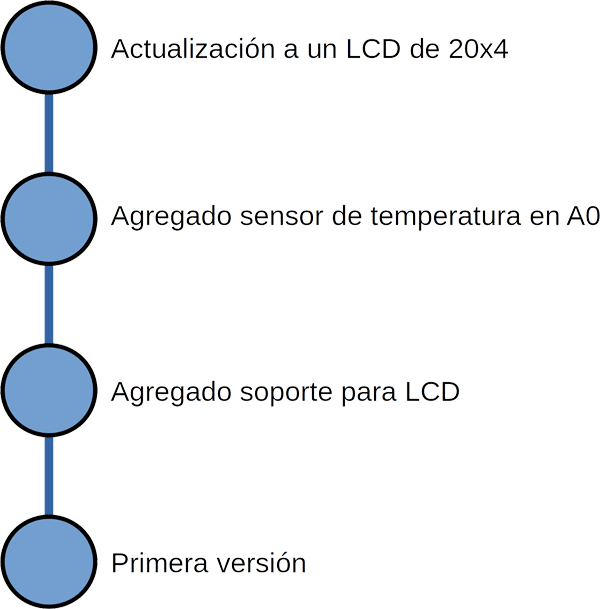
\includegraphics[scale=.23]{commit.png} 
\column{0.6\textwidth}
\begin{itemize}
\justifying
 \item Cada uno de los nodos representa un cambio confirmado (commit).
 \item A una sucesión de commits se le conoce como rama (branch)
 \item La rama principal del proyecto es la rama master
 \item La master es la rama estable, por tanto se trata de no modificarla.
 \item Para hacer cambios sin modificar la master, es posible crear una nueva rama.
\end{itemize}
\end{columns}
\end{frame}


\begin{frame}{¿Qué es Git?\hfill 
\includegraphics[scale=.1]{eciem.png}}
\begin{columns}
\column{0.4\textwidth}
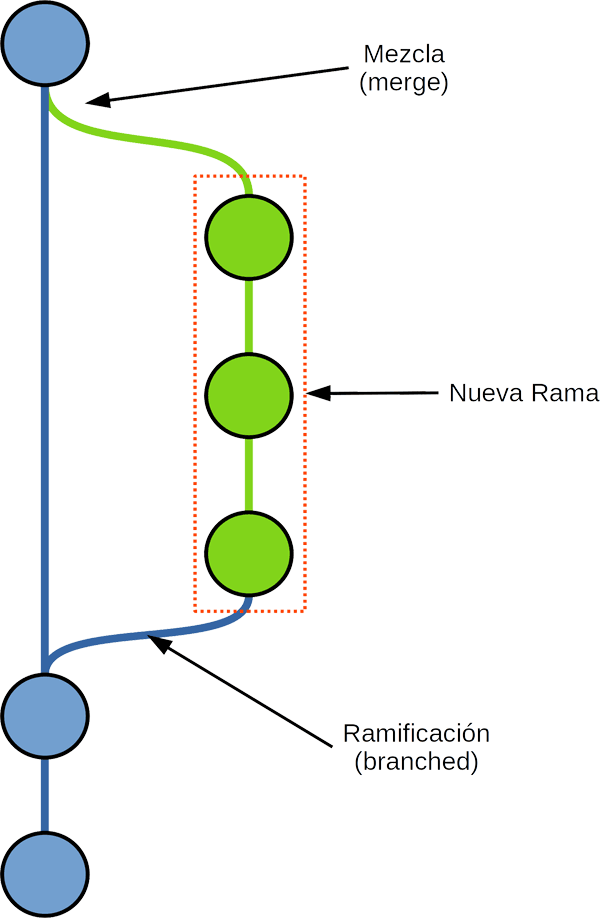
\includegraphics[scale=.22]{commit_rama.png} 
\column{0.6\textwidth}
\begin{itemize}
\justifying
 \item Cada uno de colaboradores puede tener una rama propia y modificar el proyecto.
 \item Cada una de las ramas tendrá su propia historia.
 \item Los cambios en las ramas son independientes de la master.
 \item La master es la rama estable, por tanto el master es siempre estable.
 \item Para incorporar los cambios al master se debe solicitar un merge
\end{itemize}
\end{columns}
\end{frame}

\begin{frame}{¿Qué es GitHub?\hfill 
\includegraphics[scale=.1]{eciem.png}}
\begin{columns}
\column{.8\textwidth}
 \begin{itemize}
 \justifying
\item Es una plataforma de desarrollo colaborativo para alojar y gestionar proyectos utilizando el sistema de control de versiones Git.
 \end{itemize}

\column{.2\textwidth}

\includegraphics[scale=.027]{github.png}  
\end{columns}
\begin{itemize}
\justifying
\item Se utiliza principalmente para la creación de código fuente (código simple o un programa completo)
\item GitHub ofrece rasgos similares a los de una red social: Se puede seguir un desarrollador, un proyecto, un tipo de programación 
\item La plataforma permite que  cualquier persona  sea capaz visualizar el código y colaborar con su desarrollo, es decir, máxima expresión del ``open source''
\end{itemize}
\end{frame}

\begin{frame}{¿Para qué me sirve GitHub?\hfill 
\includegraphics[scale=.1]{eciem.png}}

\end{frame}

\begin{frame}{¿Qué es GitHub Desktop? \hfill 
\includegraphics[scale=.1]{eciem.png}}
\begin{center}

\includegraphics[scale=.21]{desktop.png} 
\end{center}%
\begin{itemize}
\justifying
\item Git se utiliza mediante linea de comandos en el terminal o consola
\item GitHub es Git, por tanto, las lineas de comanda funcionan,  pero se puede utilizar mediante un web browser
\item GitHub Desktop es una aplicación que te habilita para interactuar con GitHub utilizando una GUI en vez de la línea de comandos o un web browser. 
\item Es un facilitador de uso de repositorios, es decir tenemos las bondades del Git sin usar comandos.
\end{itemize}
\end{frame}

\section{Usando GitHub}
\begin{frame}{Requisitos \hfill 
\includegraphics[scale=.1]{eciem.png}}
\begin{enumerate}
\item Cree su cuenta en GitHub accediendo \href{https://github.com/login}{aquí}
\item Descargue e instale Git desde \href{https://git-scm.com/downloads}{aquí}
\item Descargue e instale GitHub Desktop desde \href{https://desktop.github.com/}{aquí}
\end{enumerate}
\end{frame}


\begin{frame}{Acciones básicas \hfill 
\includegraphics[scale=.1]{eciem.png}}
Existen un conjunto de acciones básicas que se deben conocer al trabajar con repositorios:
\begin{itemize}
\justifying
\item \textbf{pull}:
\item \textbf{commit}:
\item \textbf{push}:
\item \textbf{clone}:
\item \textbf{fork}:
\end{itemize}
\end{frame}

\begin{frame}{Trabajemos \hfill 
\includegraphics[scale=.1]{eciem.png}}
\begin{itemize}
\item Crear un repositorio usando web browser
\item Crear desde GitHub Desktop
\item Clonar el repositorio
\item Modificar un archivo y hacer un Commit
\item Hacer un Push
\item Modificar un archivo en linea y hacer un pull
\end{itemize}
\end{frame}

\end{document}